\documentclass[10pt,twocolumn,letterpaper]{article}

\usepackage{cvpr}
\usepackage{times}
\usepackage{epsfig}
\usepackage{graphicx}
\usepackage{amsmath}
\usepackage{amssymb}
\usepackage{booktabs}
\usepackage{xcolor}
\usepackage{enumitem}
\usepackage{float}

\setlist[itemize]{noitemsep}

% Tighter spacing around floats (figures/tables) to reclaim vertical space
\setlength{\textfloatsep}{6pt plus 2pt minus 2pt}
\setlength{\floatsep}{6pt plus 2pt minus 2pt}
\setlength{\intextsep}{6pt plus 2pt minus 2pt}
\setlength{\abovecaptionskip}{2pt}
\setlength{\belowcaptionskip}{0pt}


% \teamtodo{...}: red placeholder text for sections the team still needs to write.
% Search for "teamtodo" to find every spot that needs human-written content.
\newcommand{\teamtodo}[1]{\textcolor{red}{\textbf{[TODO]} #1}}

% Include other packages here, before hyperref.
\usepackage[pagebackref=true,breaklinks=true,letterpaper=true,colorlinks,bookmarks=false]{hyperref}

\cvprfinalcopy % *** Uncomment this line for the final submission

\def\cvprPaperID{****} % *** Enter the CVPR Paper ID here
\def\httilde{\mbox{\tt\raisebox{-.5ex}{\symbol{126}}}}

\ifcvprfinal\pagestyle{empty}\fi
\begin{document}

%%%%%%%%% TITLE
\title{From Show and Tell to Attention and Transformers:\\
An Empirical Study of Architecture for Image Captioning}

\author{Hao Yang\\
Georgia Institute of Technology\\
{\tt\small hphd9@gatech.edu}
\and
Qun Wei\\
Georgia Institute of Technology\\
{\tt\small qwei49@gatech.edu}
\and
Oscar A. Martinez\\
Georgia Institute of Technology\\
{\tt\small omartinez33@gatech.edu}
\and
Yongjian Wei\\
Georgia Institute of Technology\\
{\tt\small ywei364@gatech.edu}
}

\maketitle
%\thispagestyle{empty}

%%%%%%%%% ABSTRACT
\begin{abstract}
   Image captioning requires effective integration of visual
   understanding and natural language generation. In this work, we
   propose a unified image captioning framework for controlled
   comparison of visual representations and decoding architectures. A
   pretrained ResNet-50~\cite{he2016deep} CNN encoder extracts global
   and spatial image features, which are combined with LSTM,
   attention-based LSTM, and Transformer decoders to form four model
   variants. The classical Show and Tell~\cite{vinyals2015show} model
   is used as the baseline, while the other variants introduce
   spatial attention and Transformer-based
   decoding~\cite{vaswani2017attention}. Experiments on the
   Flickr8K~\cite{hodosh2013framing} dataset using standard metrics
   (BLEU, METEOR, ROUGE-L, CIDEr) show that spatial features improve
   visual grounding, and Transformer decoders further enhance
   performance by better modeling contextual dependencies.
\end{abstract}

%%%%%%%%% BODY TEXT
\section{Introduction / Background / Motivation}

\subsection{Project Objective: Automatic Image Description}
The goal of this project is to build a system that can look at a
photograph and automatically generate a natural, human-like sentence
describing what is happening in it. We aim to compare several
different system designs under the exact same setup to identify which
one writes the most accurate and descriptive captions.

\subsection{Current Practice and Key Limitations}
Current image captioning models usually use an image encoder and a
text decoder, using attention mechanisms~\cite{xu2015show} to focus on
important image regions. However, these systems have limitations; they
frequently produce generic or inaccurate captions, miss fine visual
details, and are sensitive to internal architecture choices such as
hidden size, layers, attention design, dropout, learning rate, and
decoding strategy.

\subsection{Impact and Motivation}
Solving this problem matters because countless images online lack
useful text descriptions. A successful automated model greatly
improves internet accessibility for visually impaired users, enhances
image search capabilities, and helps organize large visual datasets.
Furthermore, it makes image data much more useful in downstream
applications that rely on combining both visual and textual
information.

\subsection{Dataset Details}
All experiments were conducted using Flickr8k
dataset~\cite{hodosh2013framing}, which is partitioned into 6k
training images, 1k validation images and 1k test images. While larger
datasets exist for image captioning task, Flickr8k was specifically
selected to achieve an optimal balance between achieving meaningful
model performance and maintaining manageable computation times during
the iterative hyperparameter tuning phase.

%-------------------------------------------------------------------------
\section{Approach}

\subsection{Overall Framework}
Figure~\ref{fig:framework} illustrates the unified image captioning
framework, which follows a standard encoder-decoder paradigm. A
pretrained ResNet-50~\cite{he2016deep} is used as the shared visual
encoder to extract image representations, while a sequence decoder
generates captions in an autoregressive, word-by-word manner. From
the encoder, two types of visual features are derived: a global
feature obtained via global average pooling, and spatial features
extracted from the final convolutional feature map that preserve
region-level information. On the decoder side, we consider three
architectures: LSTM, attention-based LSTM, and Transformer. By
combining different visual representations with different decoders,
we construct four model variants (M1 to M4), as summarized in
Table~\ref{tab:configs}. The global feature $+$ LSTM model (M1)
corresponds to the Show and Tell~\cite{vinyals2015show} framework and
serves as our baseline, while the other variants introduce spatial
attention or Transformer-based decoding.

This unified design enables controlled comparisons along two key
dimensions: visual representation (global vs.\ spatial features) and
decoding architecture (LSTM, attention-based LSTM, and Transformer),
allowing us to systematically evaluate their impact on caption
generation performance.

\begin{figure}[t]
\begin{center}
% \fbox{\rule{0pt}{1.6in} \rule{0.9\linewidth}{0pt}}
   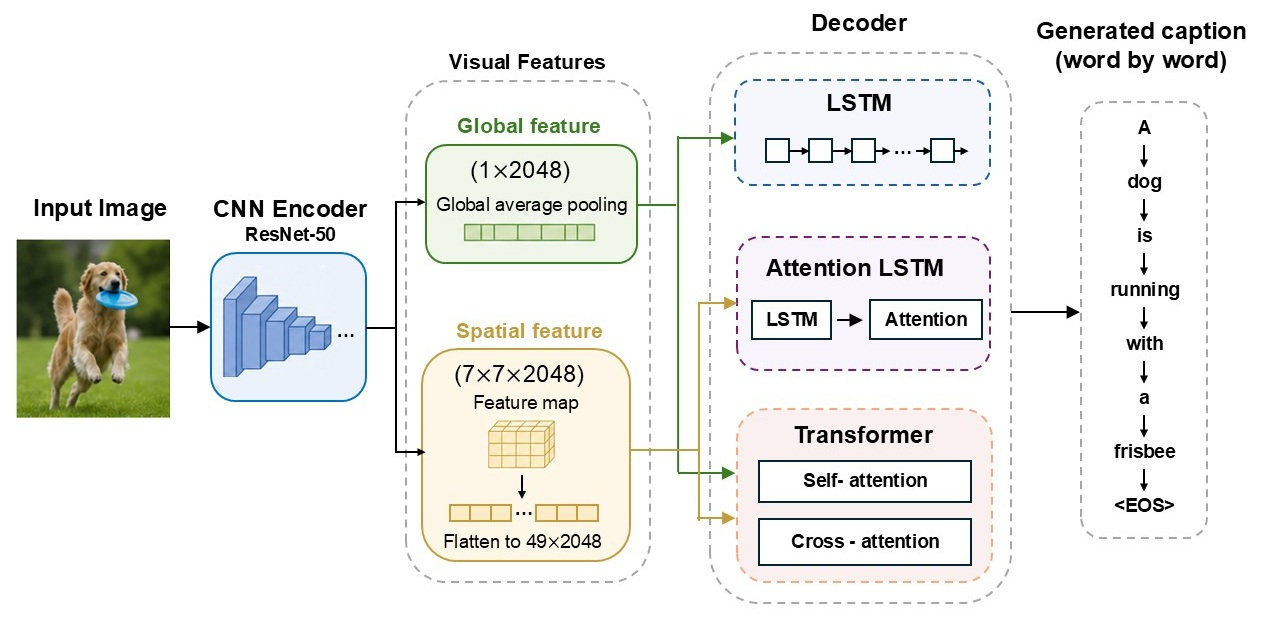
\includegraphics[width=0.95\linewidth]{figures/architecture.png}
   \caption{\footnotesize Overview of the unified image captioning
    framework with interchangeable encoder and decoder components.}
\label{fig:framework}
\end{center}
\end{figure}

\begin{table}[t]
\begin{center}
\small
\setlength{\tabcolsep}{4pt}
\begin{tabular}{@{}llll@{}}
\toprule
Model & Encoder & Decoder & Description \\
\midrule
M1 & Global  & LSTM           & Show and Tell baseline \\
M2 & Spatial & Attn-LSTM      & Attention-based LSTM \\
M3 & Spatial & Transformer    & Transformer w/ spatial \\
M4 & Global  & Transformer    & Transformer w/ global \\
\bottomrule
\end{tabular}
\caption{\footnotesize Model Configurations.}
\label{tab:configs}
\end{center}
\end{table}

\subsection{Visual encoding}
We use a pretrained ResNet-50~\cite{he2016deep} as the shared visual
encoder for all models. Show-and-Tell~\cite{vinyals2015show} originally
used an Inception-based encoder; we adopt ResNet-50 for its stronger
representations, broad adoption, and modular compatibility across model
variants. ImageNet~\cite{deng2009imagenet} pretrained weights are used
with the backbone frozen during training.

Two visual representations are derived from the same backbone.
\textbf{Spatial encoding} uses the output of the final convolutional
block before global average pooling, producing a $7\times 7\times 2048$
feature map that is reshaped into 49 region features and projected to
$(49, 512)$ for attention-based decoding. \textbf{Global encoding} is
derived from the same spatial representation by average-pooling the 49
projected region features into a single 512-D image vector. The two
representations capture complementary information: global features
encode holistic scene semantics, while spatial features preserve
region-level information for object-word alignment. Spatial features
are expected to benefit caption quality through finer visual grounding,
whereas global features provide a simpler, strong baseline.

\subsection{Caption decoding architectures}
All models formulate caption generation as autoregressive
next-token prediction conditioned on image features and previously
generated words. Three decoder families are compared:

\begin{itemize}
    \item \textbf{LSTM (M1)} follows the encoder-decoder formulation
    of Show and Tell~\cite{vinyals2015show}: a global image feature
    initializes the recurrent decoder's hidden state, and tokens are
    generated step by step.
    \item \textbf{Attention-LSTM (M2)} extends the recurrent decoder
    with soft visual attention~\cite{xu2015show} over the 49 spatial
    regions at each step, enabling dynamic region selection during
    generation.
    \item \textbf{Transformer (M3, M4)} replaces recurrence with stacked
    masked self-attention and cross-attention layers~\cite{vaswani2017attention}.
    Caption tokens attend both to previous words (causal self-attention)
    and to encoded visual regions (cross-attention). M3 uses spatial
    visual features; M4 uses the same global feature as M1, isolating
    the effect of decoder family under a fixed visual representation.
\end{itemize}

These architectures span increasing modeling capacity, from sequential
recurrence, to recurrence with attention, to fully attention-based
decoding, enabling a controlled comparison of decoder design under
shared training and evaluation settings.

\subsection{Word Embeddings}
Three word embedding strategies are considered: \textbf{random
initialization}, \textbf{pretrained GloVe~\cite{pennington2014glove}
embeddings with frozen weights}, and \textbf{pretrained GloVe
embeddings with fine-tuning}. In the first setting, embeddings are
learned from scratch during training, serving as a baseline without
external linguistic knowledge. In the second setting, embeddings are
initialized using pretrained GloVe vectors (trained on large-scale
text corpora to capture global word co-occurrence statistics) and
kept fixed, providing stable semantic representations while reducing
overfitting. In the third setting, pretrained embeddings are further
fine-tuned, allowing adaptation to the captioning task and
potentially improving alignment between visual and textual features.

The pretrained GloVe embeddings are 300-dimensional, while the model
embedding size is 512. To address this mismatch, a linear projection
layer is applied to map the embeddings into the model space. To
ensure fair comparison, all models share the same vocabulary and
embedding dimensionality, and only the embedding initialization and
trainability are varied. Pretrained embeddings are expected to
provide improvements over random initialization, while the additional
benefit of fine-tuning may be limited due to the limited size of the
training data.

\subsection{Evaluation Metrics}
Caption quality is evaluated using four standard metrics:
\textbf{BLEU}~\cite{papineni2002bleu},
\textbf{METEOR}~\cite{banerjee2005meteor},
\textbf{ROUGE}-L~\cite{lin2004rouge}, and
\textbf{CIDEr}~\cite{vedantam2015cider}, which are widely adopted in
prior image captioning studies. BLEU measures n-gram precision
between generated captions and reference captions, emphasizing local
word overlap. METEOR incorporates both precision and recall with
additional alignment mechanisms such as stemming and synonym
matching, making it more sensitive to semantic similarity. ROUGE-L is
based on the longest common subsequence and captures sentence-level
structure and fluency. CIDEr measures consensus between generated
captions and multiple references using TF-IDF weighting, emphasizing
the importance of informative and distinctive words.

Among these metrics, CIDEr is considered the primary metric in this
work, as it is specifically designed for image captioning and better
reflects human judgment by accounting for consensus across multiple
references. BLEU and ROUGE-L provide complementary insights into
lexical overlap and structural similarity, while METEOR offers
additional sensitivity to semantic variations. All metrics are
reported to provide a comprehensive evaluation of model performance.

\section{Experiments and Results}

\subsection{Experimental setup and model configurations}

\noindent\textbf{Code repositories and prior sources.}
The full implementation is available at our
\href{https://github.com/haoyang86/ImageCaptioning/tree/main}{GitHub
repository}. The training pipeline, encoders, attention module,
Transformer decoder layer, and evaluation utilities were written from
scratch in PyTorch; we referenced patterns from our own prior CS 7643
coursework (Assignments 2 and 3) for scaffolding such as training-loop
structure and evaluation harnesses, but no code was copied verbatim.
Third-party dependencies are limited to \texttt{torchvision}'s
ImageNet-pretrained ResNet-50 weights, the standard NLTK BLEU/METEOR
implementations, and a CIDEr scorer adapted from the public
coco-caption toolkit. This report is built from the course-provided
\href{https://www.overleaf.com/project/5f5ec061aa94370001943266}{\LaTeX{}
template}.

% Commented this out as its standard practice and we need space
% ; the preamble additionally reuses small formatting helpers
% (custom commands, list spacing, table float conventions) accumulated
% across the author's prior coursework, but no substantive content was
% carried over.

\noindent\textbf{Dataset.}
Flickr8k~\cite{hodosh2013framing} (partition into training-6k,
dev-1k, and test-1k data).

\noindent\textbf{Loss function.} All models were trained to minimize the
cross-entropy loss, which calculates the per-token probability error
of the generated caption against the ground truth.

\noindent\textbf{Optimizer.} The AdamW~\cite{loshchilov2019decoupled}
optimizer was preferred over standard Adam. AdamW decouples weight
decay from the gradient update step, which is recommended for
training complex sequence models like transformer and LSTM, leading
to better generalization.

\noindent\textbf{Transfer Learning.} Due to smaller dataset (Flickr8k),
transfer learning was utilized to accelerate convergence across all
the models. The weights of the Resnet-50 encoder were strictly frozen
during training. The model primarily focuses on optimizing the
decoder's ability to map established visual representations to text.

\begin{table}[t]
\begin{center}
\setlength{\tabcolsep}{4pt}
\begin{tabular}{lcccccc}
\toprule
Model & LR & WD & Hid. & Lyrs. & Heads & Drop. \\
\midrule
M1 & 1e-4 & 0.05 & 512 & 2 & NA  & 0.1 \\
M2 & 1e-4 & 0.05 & 512 & 1 & 1   & 0.1 \\
M3 & 1e-4 & 0.05 & 512 & 4 & 8   & 0.3 \\
M4 & 1e-4 & 0.05 & 512 & 4 & 8   & 0.3 \\
\bottomrule
\end{tabular}
\caption{\footnotesize Model-specific best hyperparameters.
WD: weight decay; Hid.: hidden/dim; Lyrs.: layers; Drop.: dropout.
All models are trained for 10 epochs with batch size 16.}
\label{tab:hparams}
\end{center}
\end{table}

\noindent\textbf{Hyperparameter Tuning Strategy.} The hyperparameters were
refined through iterative tuning, with specific attention to
regularization mainly due to relatively small size of Flickr8k
dataset use (Table~\ref{tab:hparams}):
\begin{itemize}
   \setlength\itemsep{0.5em}
    \item \textbf{Batch size:} A batch size of 16 was utilized.
    During tuning, smaller batch size provided a regularization
    effect through slightly noisier gradient updates, which helped
    the models escape sharp local minima.
    \item \textbf{Learning Rate Scheduler:} A learning rate scheduler
    was implemented, utilizing a warmup phase (first 2 epochs)
    followed by annealing. The warmup phase was to prevent early
    divergence, especially for transformer decoder, while the
    annealing allowed the optimizer to smoothly settle into the
    final optimal weights in the last few epochs.
    \item \textbf{Regularization:} to combat overfitting on the
    small dataset, a dropout rate ranging from 0.1 to 0.3 were
    applied to the encoder and decoder models respectively. And a
    weight decay of 0.05 was enforced via the AdamW optimizer to
    penalize overly large network weights.
\end{itemize}

\noindent\textbf{Training results.} Figure~\ref{fig:loss} illustrates the
loss curves of two examples (M1 and M3) across 10 epochs. The
baseline model (global $+$ LSTM) demonstrates stable convergence, with
training and validation loss aligning closely after 10 epochs.
Conversely, despite aggressive regularization, the more complex
Transformer exhibited a divergence between training and validation
loss, which is typical for high-capacity models on small datasets.
However, the Transformer ultimately achieved better overall performance
compared to LSTM.

\begin{figure}[t]
\begin{center}
   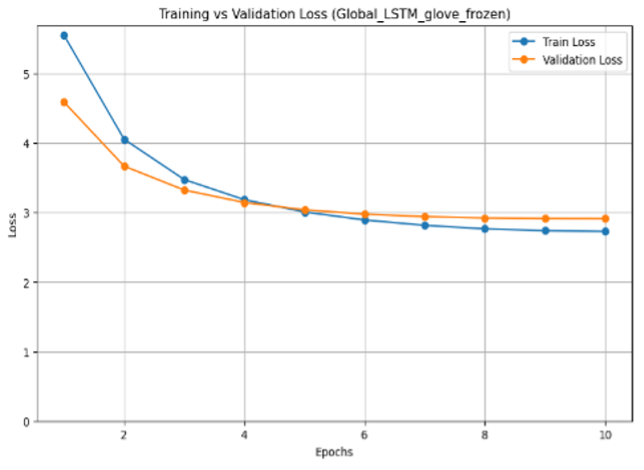
\includegraphics[width=0.48\linewidth]{figures/plot01.png}\hfill
   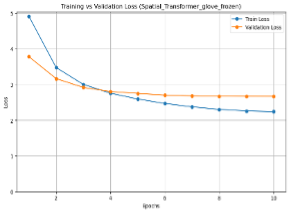
\includegraphics[width=0.48\linewidth]{figures/plot02.png}
   \caption{\footnotesize Training convergence comparison between
   M1 (left) and M3 (right).}
\label{fig:loss}
\end{center}
\end{figure}

\subsection{Architecture Comparison}
This section evaluates the four model variants to analyze how
specific architectural choices influence caption quality. To ensure
optimal sequence generation, all evaluation metrics were calculated
using beam search decoding strategy. Table~\ref{tab:arch} summarizes
the quantitative results for each model.

A consistent observation across the result is the impact of Visual
Representation: Global vs Spatial (M1 vs.\ M2 \& M4 vs.\ M3):
preserving spatial features significantly improves performance for
both LSTM and transformer based decoders.
\begin{itemize}
    \item (M1 vs.\ M2): the baseline model forces the entire image
    into a single global vector, discarding localized visual details.
    By transitioning to CNN spatial features paired with an
    Attention-LSTM (M2), the decoder has the ability to focus on
    specific image regions for each generated word. This localized
    visual grounding generates higher caption accuracy of CIDEr score
    from 0.37 to 0.42.
    \item (M3 vs.\ M4): the transformer decoder shows a similar
    reliance on spatial information. The global feature discards the
    visual region details that cross-attention mechanisms in
    transformer decoder are designed to exploit. It results in more
    generalized and less accurate captions. On the other hand, with
    spatial feature map provided, the transformer can align distinct
    image regions with visual tokens, allowing the generated text to
    be tightly grounded to specific objects and backgrounds. As a
    result, M3 pushes the CIDEr score to a project-high of 0.47.
\end{itemize}

For the impact of decoder architecture, M3 outperforms M2 because the
Transformer decoder uses the same spatial image features more
effectively than the Attention-LSTM decoder. In M2, caption
generation depends on a recurrent hidden state, so visual and
language context must be carried forward step by step. This can limit
how well the decoder preserves earlier information, especially when
generating longer phrases. In contrast, M3 uses masked self-attention,
allowing each word position to directly reference previous caption
tokens, while cross-attention links those tokens to spatial image
regions. This structure gives M3 a more flexible way to model object
relationships, phrase structure, and image-text alignment. Therefore,
with the same spatial encoder input, M3 produces more coherent and
better-grounded captions than M2.

\begin{table}[t]
\begin{center}
\setlength{\tabcolsep}{4pt}
\begin{tabular}{lccccccc}
\toprule
Model & B-1 & B-2 & B-3 & B-4 & MET. & R-L & CIDEr \\
\midrule
M1 & 0.56 & 0.37 & 0.24 & 0.15 & 0.36 & 0.44 & 0.37 \\
M2 & 0.58 & 0.40 & 0.26 & 0.17 & 0.37 & 0.46 & 0.42 \\
M3 & 0.58 & 0.40 & 0.27 & 0.18 & 0.38 & 0.46 & 0.47 \\
M4 & 0.57 & 0.39 & 0.25 & 0.17 & 0.37 & 0.45 & 0.43 \\
\bottomrule
\end{tabular}
\caption{\footnotesize Quantitative architecture comparison (best
hyperparameter model). B-$n$: BLEU-$n$, MET.: METEOR, R-L: ROUGE-L.}
\label{tab:arch}
\end{center}
\end{table}

\subsection{Embedding Comparison}
To assess the impact of prior semantic knowledge on the image caption
generation process, three models, baseline (M1: Global$+$LSTM), M2
(Spatial$+$Attention-LSTM) and M3 (Spatial$+$Transformer), were
evaluated across three word embedding configurations. Although the
experimental results in Tables~\ref{tab:emb-m1},
\ref{tab:emb-m2}, and~\ref{tab:emb-m3} demonstrate that the
introduction of pre-trained GloVe embeddings yield negligible
improvements across all architectures, the underlying reasons for
this lack of impact could differ.

\begin{table}[t]
\begin{center}
\small
\setlength{\tabcolsep}{3pt}
\begin{tabular}{lccccccc}
\toprule
Embedding & B-1 & B-2 & B-3 & B-4 & MET. & R-L & CIDEr \\
\midrule
Random         & .568 & .379 & .245 & .155 & .355 & .445 & .370 \\
GloVe frozen   & .562 & .372 & .241 & .152 & .356 & .442 & .373 \\
GloVe finetune & .558 & .367 & .237 & .155 & .355 & .445 & .370 \\
\bottomrule
\end{tabular}
\caption{\footnotesize Metrics results for baseline M1 (Global$+$LSTM).}
\label{tab:emb-m1}
\end{center}
\end{table}

\begin{table}[t]
\begin{center}
\small
\setlength{\tabcolsep}{3pt}
\begin{tabular}{lccccccc}
\toprule
Embedding & B-1 & B-2 & B-3 & B-4 & MET. & R-L & CIDEr \\
\midrule
Random         & .546 & .369 & .243 & .154 & .368 & .454 & .417 \\
GloVe frozen   & .572 & .386 & .255 & .165 & .368 & .452 & .421 \\
GloVe finetune & .573 & .389 & .260 & .169 & .370 & .455 & .422 \\
\bottomrule
\end{tabular}
\caption{\footnotesize Metrics results for M2 (Spatial$+$LSTM Attention).}
\label{tab:emb-m2}
\end{center}
\end{table}

\begin{table}[t]
\begin{center}
\small
\setlength{\tabcolsep}{3pt}
\begin{tabular}{lccccccc}
\toprule
Embedding & B-1 & B-2 & B-3 & B-4 & MET. & R-L & CIDEr \\
\midrule
Random         & .581 & .398 & .271 & .181 & .383 & .465 & .473 \\
GloVe frozen   & .582 & .398 & .271 & .183 & .379 & .463 & .467 \\
GloVe finetune & .587 & .404 & .275 & .184 & .380 & .463 & .478 \\
\bottomrule
\end{tabular}
\caption{\footnotesize Metrics results for M3 (Spatial$+$Transformer).}
\label{tab:emb-m3}
\end{center}
\end{table}

For baseline M1 and M2 architecture, the primary limitation is
architecture rather than semantic. M1 compresses the visual input
into a single global vector and the LSTM decoder lacks the visual
context to effectively align with the rich, pre-existing semantic
space provided by GloVe. M2 introduces spatial feature and attention
mechanism, the performance from random to GloVe embeddings shows
improvements in BLEU and remain marginal in the other metrics.
Conversely, for the M3 architecture, the negligible difference
between different embeddings indicates a limitation of data scale.
Because the training set is relatively small, the transformer
reaches the performance ceiling and begins to overfit as illustrated
in the earlier training results. Therefore, it does not fully exploit
the high-dimensional semantic spaces provided by the GloVe
embeddings, and embeddings don't play a decisive factor in the
results.

\subsection{Qualitative Analysis}
To further understand model behavior beyond quantitative metrics, we
present qualitative comparisons across three levels of difficulty:
easy, medium, and challenging cases, as shown in
Figure~\ref{fig:qual}.

In easy cases (Figure~\ref{fig:qual}, left), all models generate
nearly identical and accurate captions, correctly identifying the
main object and action (e.g., dog and running in snow). This suggests
that when visual cues are salient and unambiguous, architectural
differences have minimal impact on performance. In medium cases
(Figure~\ref{fig:qual}, middle), all models correctly capture the
main scene but differ in the level of detail. For example, while
all models recognize a dog playing in water, M1 describes only the
general activity (``playing in the water'') and misses the key
object (tennis ball). M2 captures the tennis ball but omits the
water context. In contrast, M3 and M4 incorporate both the tennis
ball and water, with M4 further including attribute-level details
such as color. This demonstrates that models with stronger
representation and decoding capacity produce more complete and
descriptive captions. In challenging cases (Figure~\ref{fig:qual},
right), all models fail to fully capture the ground-truth semantics,
but exhibit distinct error patterns. For instance, none of the
models detect the small object or the interaction (watching),
instead generating coarse descriptions such as ``people standing
near water.'' M1 and M4 produce plausible but generic captions, M2
partially improves environmental understanding (e.g., ``lake''),
while M3 generates an unrelated scene (e.g., involving a building),
indicating hallucination. These differences highlight limitations in
capturing fine-grained details and interactions.

Overall, as task difficulty increases, model differences become more
pronounced. Transformer-based models tend to produce richer
descriptions in moderately complex scenarios but may also introduce
instability in difficult cases. This behavior is likely amplified by
the limited size of the dataset (Flickr8k), which can lead to
reliance on frequent patterns and reduced robustness.

%-------------------------------------------------------------------------
\section{Discussion and Conclusion}

Our controlled experiments with four different models reveals a
fundamental tradeoff between complexity and representation power.
The baseline M1 (Global$+$LSTM) is computationally efficient but
lacks complexity and capacity, resulting in worst performance in the
comparison. M2 adds complexity by using attention mechanisms to
align text tokens with image local regions, and the performance sits
in the middle ground. M3 (Spatial$+$Transformer) achieves the
highest metrics but easy to overfit with small training data. M4
underperformed compared to M3 due to inefficient use of
cross-attention with compressed global visual feature.

This project successfully evaluated four different architectures to
isolate the impact of visual representation and decoding architecture
in the image captioning task. The results clearly demonstrate that
preserving spatial visual features is critical for accurate
image-text alignment. Furthermore, with rich spatial features from
encoder, the Transformer architecture outperforms traditional
attention-LSTM approach, by utilizing masked self-attention and
cross-attention to generate highly contextual captions for image.

\teamtodo{The CS 7643 rubric expects the report to also address
deep-learning-specific reflection questions: how the model structure
reflects the problem structure; which parts of the model have learned
parameters and which do not; how the data is pre/post-processed;
whether the model overfit and how it generalized; what
hyperparameters mattered and how they were chosen; what framework
was used; what existing code or models were used as starting points;
and potential future work. v2 does not address these directly; add
a short paragraph (or expand this section) to cover them.}

%-------------------------------------------------------------------------


\begin{figure*}[h]
\begin{center}
% \fbox{\rule{0pt}{2.2in} \rule{0.95\linewidth}{0pt}}
   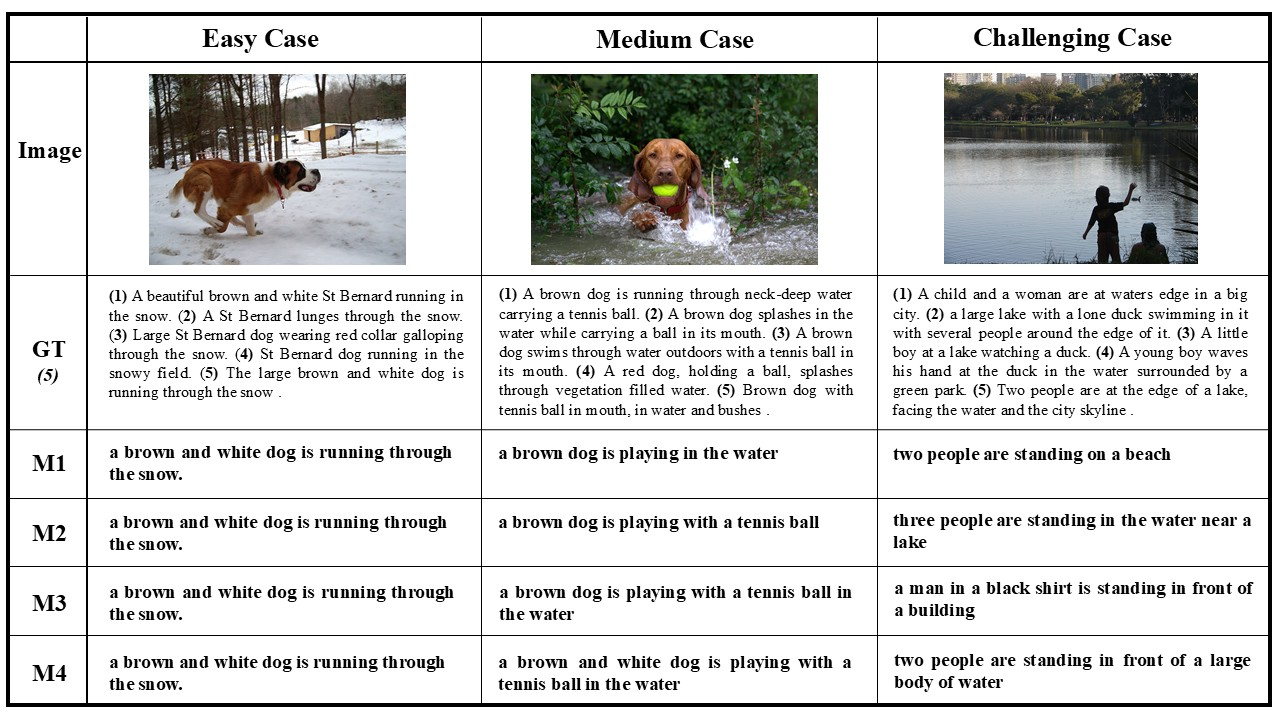
\includegraphics[width=0.95\linewidth]{figures/comparison.png}
   \caption{\footnotesize Qualitative comparison of generated
   captions across three difficulty levels (easy, medium, and
   challenging).}
\label{fig:qual}
\end{center}
\end{figure*}

\section*{Work Division}

Work was distributed so that every member contributed to both
implementation and writing. Model variants were primarily owned as
follows: Hao led M3, Yongjian led M2, and Oscar led the initial M1
and M4 implementations; Qun and Yongjian jointly developed the LSTM
attention decoder shared across variants. Cross-cutting work (the
unified codebase, embedding ablation, evaluation harness, and
\LaTeX{} transcription) and individual report sections were divided
across the team as detailed in Table~\ref{tab:contributions}.

\begin{table}[H]
\begin{center}
\small
\begin{tabular}{@{}lp{5.5cm}@{}}
\toprule
Members & Contributions \\
\midrule
Hao Yang & Developed the implementation of the M3 model, beam search decoding, and evaluation metrics. 
   Contributed to the design of the overall codebase structure and the unification of all four models (M1 to M4). 
   Ran experiments for the M3 model. 
   Initiated report organization and completed Abstract, Section 2, and Section 3.4. \\
Yongjian Wei & 
  M2: Spatial encoder and LSTM attention code development.
  Run experiments for M2 model.
  Report writing section 1, section 3.2. \\
Qun Wei & 
  Co-development of multi-layers LSTM attention decoder with Yongjian.
  Implemented Global encoder and a unified model for M1, M2, M3, and M4 for team collaboration.
  Run experiments for embeddings for all models.
  Report writing section 3.1, 3.3 and 4. \\
Oscar A.~Martinez & 
  Transcription of report from Word to \LaTeX, and overall report formatting.
  Initial M1 and M4 code development.
  Creation of Optuna scripts for hyperparameter tuning (M1 and M4). \\
\bottomrule
\end{tabular}
\caption{\footnotesize Contributions of team members.}
\label{tab:contributions}
\end{center}
\end{table}

%-------------------------------------------------------------------------

\clearpage 
{\small
\bibliographystyle{ieee_fullname}
\bibliography{egbib}
}

\end{document}
